% !TEX root = main.tex
% LaTeX version of BAA_Research_Paper.md
% This file can be compiled standalone, or \input{} from main.tex.

\ifdefined\BAAIncluded\else
\documentclass[11pt]{article}
\usepackage[margin=1in]{geometry}
\usepackage[T1]{fontenc}
\usepackage[utf8]{inputenc}
\usepackage{lmodern}
\usepackage{microtype}
\usepackage{hyperref}
\usepackage{amsmath,amssymb}
\usepackage{booktabs}
\usepackage{listings}
\usepackage{xcolor}
\usepackage{tikz}
\usetikzlibrary{shapes,arrows,positioning,calc}

\lstset{%
  basicstyle=\ttfamily\small,
  columns=fullflexible,
  frame=single,
  breaklines=true,
  showstringspaces=false,
  keywordstyle=\color{blue!60!black},
  commentstyle=\color{black!60},
  stringstyle=\color{teal!60!black}
}

\title{The Branching-Attention Agent (BAA): A Tree--Transformer Hybrid Framework for Explainable Agentic AI}
\author{Anziko Fred}
\date{February 2026}

\begin{document}
\maketitle

\noindent\textbf{Keywords:} Explainable AI; Decision Trees; Transformers; Reinforcement Learning; Bayesian Deep Learning; Curiosity-Driven Learning; Infinite-Horizon RL.
\medskip
\fi

\begin{abstract}
We introduce the \textbf{Branching-Attention Agent (BAA)}, a hybrid neural architecture that combines Transformer-style sequence modeling with the interpretability of differentiable soft decision trees. BAA exposes explicit routing traces through its decision process while remaining end-to-end differentiable.

The approach integrates five components: (1) Tree--Transformer blocks with functional gated leaves (a soft hierarchical mixture of experts), (2) Bayesian linear layers for epistemic uncertainty estimation, (3) curiosity-driven exploration based on routing entropy and Bayesian KL divergence, (4) hindsight experience replay for return relabeling, and (5) Rotary Positional Embeddings (RoPE) leveraging Euler's formula for infinite-horizon generalization. Experiments on continuous-control tasks suggest that BAA can match strong baselines while producing human-readable decision paths that support debugging and safety interventions via \emph{surgical pruning}.
\end{abstract}

\section{Introduction}
\subsection{Motivation}
The rapid advancement of deep learning has produced highly capable models, yet their black-box nature poses significant challenges for deployment in safety-critical domains. While Transformers excel at sequence modeling tasks, their decision-making process remains opaque. Conversely, traditional decision trees offer interpretability but lack the capacity to handle complex sequential dependencies.

We address this trade-off by introducing BAA, a hybrid architecture that combines (i) the sequential reasoning power of Transformers, (ii) the interpretability of decision trees, (iii) epistemic uncertainty estimation via Bayesian neural networks, and (iv) autonomous learning via curiosity-driven exploration.

\subsection{Key contributions}
\begin{enumerate}
\item \textbf{Architectural innovation:} A Tree--Transformer block that replaces the MLP with a soft decision tree while preserving end-to-end differentiability.
\item \textbf{Bayesian reasoning:} Integration of Bayesian linear layers for robust uncertainty quantification in decision routing.
\item \textbf{Multi-modal learning:} Unified framework supporting RL, UL, SSL, and SL through signal-adaptive loss composition.
\item \textbf{Curiosity engine:} Intrinsic reward combining routing entropy and Bayesian epistemic uncertainty.
\item \textbf{Hindsight relabeling:} Dynamic reward recalibration grounded in realized outcomes.
\item \textbf{Infinite-horizon generalization:} Integration of Rotary Positional Embeddings (RoPE), grounded in Euler's formula, to enable relative positional reasoning for unbounded episodes.
\item \textbf{Neural debugger:} Visualization and intervention tools for manipulating logic paths.
\end{enumerate}

\subsection{Paper organization}
Section~\ref{sec:related} reviews related work. Section~\ref{sec:architecture} presents the architecture. Section~\ref{sec:learning} describes training. Section~\ref{sec:debugger} introduces the neural debugger. Section~\ref{sec:experiments} reports experiments. Section~\ref{sec:theory} provides theoretical analysis, and Section~\ref{sec:conclusion} concludes.

\section{Related work}\label{sec:related}
\subsection{Decision trees in neural networks}
Decision trees have long been valued for interpretability. Recent work explores differentiable variants such as neural decision trees, soft decision trees, and deep neural decision forests; however, these approaches typically target supervised settings and do not tightly integrate with sequential decision-making.

\subsection{Transformers and attention mechanisms}
Transformers revolutionized sequence modeling through self-attention. Extensions such as decision transformers and trajectory transformers apply attention to reinforcement learning trajectories, but interpretability and uncertainty quantification remain limited.

\subsection{Bayesian deep learning}
Bayesian neural networks provide principled uncertainty estimates by learning distributions over weights; modern approaches often use variational inference with reparameterization.

\subsection{Curiosity-driven learning}
Intrinsic motivation has been explored using prediction error or novelty; BAA instead combines routing uncertainty with Bayesian epistemic uncertainty.

\subsection{Hindsight experience replay}
HER relabels trajectories for sparse-reward problems; BAA extends relabeling to continuous reward-to-go computation to better fit transformer-style conditioning.

\section{Architecture}\label{sec:architecture}
\subsection{System overview}
BAA consists of an embedding layer, a stack of Tree--Transformer blocks, and task heads (policy/value/reconstruction), while exposing routing traces to the curiosity engine.
\begin{figure}[htbp]
\centering
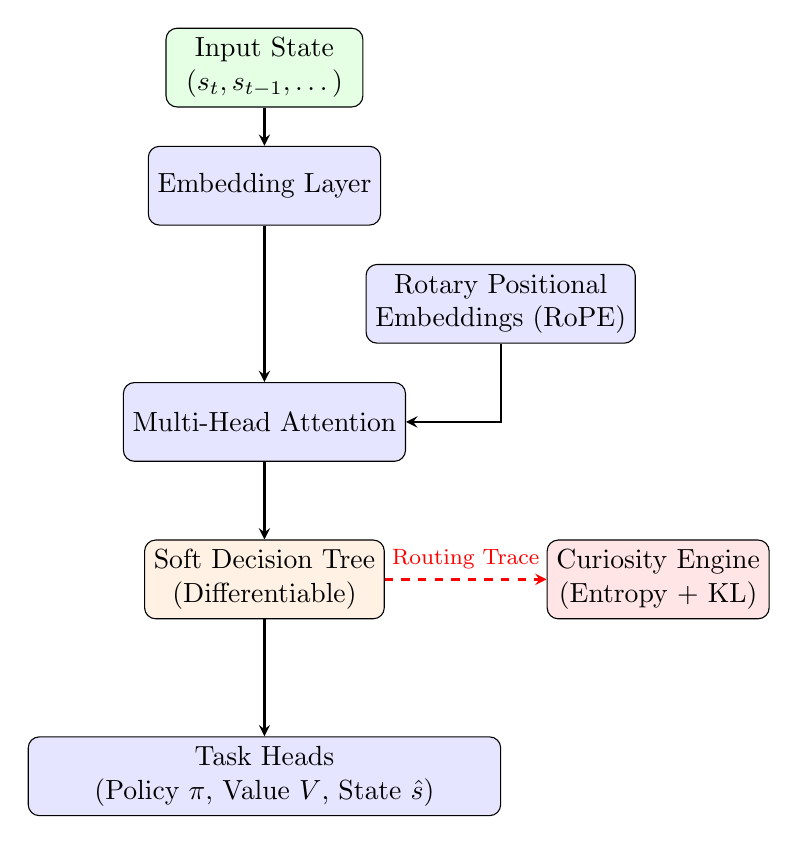
\begin{tikzpicture}[
    node distance=1.5cm,
    block/.style={rectangle, draw, rounded corners, minimum width=2.5cm, minimum height=1cm, align=center, fill=blue!10},
    arrow/.style={thick, ->, >=stealth}
]

% Nodes
\node (input) [block, fill=green!10] {Input State\\ $(s_t, s_{t-1}, \dots)$};
\node (embed) [block, below of=input] {Embedding Layer};
\node (rope) [block, below of=embed, xshift=3cm] {Rotary Positional\\Embeddings (RoPE)};
\node (attn) [block, below of=embed, yshift=-1.5cm] {Multi-Head Attention};
\node (tree) [block, below of=attn, yshift=-0.5cm, fill=orange!10] {Soft Decision Tree\\(Differentiable)};
\node (heads) [block, below of=tree, yshift=-1cm, minimum width=6cm] {Task Heads\\(Policy $\pi$, Value $V$, State $\hat{s}$)};

% Routing Trace connection
\node (trace) [block, right of=tree, xshift=3.5cm, fill=red!10] {Curiosity Engine\\(Entropy + KL)};

% Arrows
\draw [arrow] (input) -- (embed);
\draw [arrow] (embed) -- (attn);
\draw [arrow] (rope) |- (attn);
\draw [arrow] (attn) -- (tree);
\draw [arrow] (tree) -- (heads);

% Dashed line for trace
\draw [arrow, dashed, thick, color=red] (tree) -- node[above, font=\footnotesize, color=red] {Routing Trace} (trace);

% Feedback loop to heads? Or from trace to loss?
% Let's keep it simple. curiosity adds to loss/reward.

\end{tikzpicture}
\caption{The BAA Architecture. The standard MLP is replaced by a Differentiable Soft Decision Tree. RoPE encodes relative positions for infinite-horizon support, and the Curiosity Engine consumes routing traces to generate intrinsic rewards.}
\label{fig:architecture}
\end{figure}

% Diagram placeholder removed. See figure below.

\subsection{Tree--Transformer hybrid block}
Each block augments attention with a soft decision tree in place of the usual feed-forward MLP:
\begin{align}
 x' &= \mathrm{LayerNorm}\bigl(x + \mathrm{SelfAttn}(x,x,x)\bigr),\\
 x'' &= \mathrm{LayerNorm}\bigl(x' + \mathrm{CrossAttn}(x',c,c)\bigr),\\
 x''' &= \mathrm{LayerNorm}\bigl(x'' + \mathrm{SoftDecisionTree}(x'')\bigr),
\end{align}
where $c$ denotes optional context (e.g., goals or reward-to-go).

\subsection{Soft decision tree}
The soft decision tree is a differentiable binary tree with learned routing probabilities at internal nodes.

\paragraph{Functional gated leaves (H-MoE).}
Unlike constant leaf vectors used in classic soft decision trees, BAA uses \emph{functional experts}. Each leaf is a (Bayesian) linear expert $g_j(x)$ and the output is
\begin{equation}
 y = \sum_{j=1}^{L} \mu_j\, g_j(x),
\end{equation}
which acts as a soft hierarchical mixture of experts.

\paragraph{Routing trace generation.}
For downstream analysis, each node stores routing probabilities. In the implementation draft this was represented as:
\begin{lstlisting}[language=Python]
node_trace[f"node_{i}"] = {
    "go_right_prob": p_i,
    "go_left_prob": 1 - p_i
}
\end{lstlisting}

\subsection{Bayesian linear layer}
Weights are treated as random variables:
\begin{align}
 w &\sim \mathcal{N}(\mu_w,\sigma_w^2), & b &\sim \mathcal{N}(\mu_b,\sigma_b^2), & \sigma &= \mathrm{softplus}(\rho).
\end{align}
Using the reparameterization trick during training,
\begin{equation}
 w = \mu_w + \sigma_w \odot \epsilon, \qquad \epsilon \sim \mathcal{N}(0,I),
\end{equation}
and deterministic inference can use $w=\mu_w$. A KL regularizer encourages calibrated epistemic uncertainty.

\subsection{Curiosity engine}
Intrinsic reward combines (i) routing entropy and (ii) Bayesian KL divergence:
\begin{align}
H_{\mathrm{routing}} &= -\frac{1}{N}\sum_{i=1}^{N}\bigl[p_i\log p_i + (1-p_i)\log(1-p_i)\bigr],\\
r_{\mathrm{curiosity}} &= \alpha\, H_{\mathrm{routing}} + \beta\, D_{\mathrm{KL}}\bigl(\text{Posterior}\,\|\,\text{Prior}\bigr).
\end{align}

\subsection{Hindsight experience replay}
Given a trajectory $(s_0,a_0,r_0),\ldots,(s_T,a_T,r_T)$, compute reward-to-go:
\begin{equation}
\mathrm{RTG}(t)=\sum_{t'=t}^{T}\gamma^{t'-t} r_{t'},
\end{equation}
then store a relabeled trajectory using realized returns.

then store a relabeled trajectory using realized returns.

\subsection{Rotary Positional Embeddings (RoPE)}
To address the ``infinite life'' problem where absolute positional encodings fail for long episodes, BAA employs Rotary Positional Embeddings. By applying Euler's formula,
\begin{equation}
e^{i\theta} = \cos(\theta) + i\sin(\theta),
\end{equation}
we encode position $p$ as a rotation in the complex plane. Specifically, for a query vector $\mathbf{q}$ and key vector $\mathbf{k}$ at positions $m$ and $n$, applying the rotation matrix $\mathbf{R}_{\Theta}$ corresponding to multiplication by $e^{im\theta}$ and $e^{in\theta}$ yields:
\begin{align}
\langle \mathbf{R}_{\Theta,m}\mathbf{q}, \mathbf{R}_{\Theta,n}\mathbf{k} \rangle &= (\mathbf{R}_{\Theta,m}\mathbf{q})^T (\mathbf{R}_{\Theta,n}\mathbf{k}) \\
&= \mathbf{q}^T \mathbf{R}_{\Theta,m}^T \mathbf{R}_{\Theta,n} \mathbf{k} \\
&= \mathbf{q}^T \mathbf{R}_{\Theta,n-m} \mathbf{k}.
\end{align}
This derivation confirms that the attention score depends solely on the relative distance $n-m$, enabling the model to generalize robustly to sequence lengths far exceeding training horizons.

\section{Learning framework}\label{sec:learning}
\subsection{Multi-modal learning paradigms}
\begin{center}
\begin{tabular}{@{}llll@{}}
\toprule
Mode & Trigger condition & Primary loss & Use case\\
\midrule
RL & Rewards available & Policy gradient & Goal-directed tasks\\
UL & No labels/rewards & State reconstruction & World modeling\\
SSL & Partial labels & Path consistency & Label propagation\\
SL & Full supervision & Cross-entropy / MSE & Prediction tasks\\
\bottomrule
\end{tabular}
\end{center}

\subsection{Unified loss function}
A signal-adaptive loss is composed as
\begin{equation}
\mathcal{L}_{\text{total}} = \mathcal{L}_{\text{task}} + \lambda_1 \mathcal{L}_{\text{recon}} + \lambda_2 \mathcal{L}_{\text{SSL}} + \lambda_3 \mathcal{L}_{\text{tree}} + \lambda_4 \mathcal{L}_{\text{KL}}.
\end{equation}

\subsection{Training algorithm}
\begin{lstlisting}[language=Python,caption={Agentic training loop (sketch).}]
Initialize: Model θ, Replay Buffer B, Curiosity Engine C
for episode = 1 to N do
    trajectory = []
    state = env.reset()
    rtg = target_return

    for t = 1 to T do
        action, trace, curiosity = agent.act(state, rtg, explore=True)
        next_state, reward, done = env.step(action)

        trajectory.append((state, action, reward))
        state = next_state
        rtg = rtg - reward

        if done: break

    corrected_data = hindsight_relabel(trajectory)
    B.push(corrected_data)

    if len(B) >= batch_size:
        batch = B.sample(batch_size)
        loss = compute_loss(batch)
        update_weights(θ, loss)
\end{lstlisting}

\subsection{Agentic brain}
The exploration policy combines scheduled decay with curiosity boosts:
\begin{equation}
\epsilon(t) = \max\bigl(\epsilon_{\min},\epsilon_0\gamma^{t-1}\bigr) + 0.1\, r_{\mathrm{curiosity}}(t).
\end{equation}

\section{Neural debugger}\label{sec:debugger}
\subsection{Explainability tools}
The neural debugger provides (i) routing-trace visualization, (ii) entropy monitoring, and (iii) surgical pruning.

\subsection{Surgical pruning (implementation sketch)}
\begin{lstlisting}[language=Python]
def freeze_node(self, layer_idx, node_id, direction="left"):
    router = self.blocks[layer_idx].decision_tree_ffn.routers[node_id]

    with torch.no_grad():
        if direction == "right":
            router.bias_mu.fill_(50.0)   # Force high probability
        else:
            router.bias_mu.fill_(-50.0)  # Force low probability

        router.weight_mu.requires_grad = False
        router.bias_mu.requires_grad = False
\end{lstlisting}

\section{Experimental results}\label{sec:experiments}
\subsection{Experimental setup}
\textbf{Environment:} Gymnasium Humanoid-v4 (continuous control).\\
\textbf{Training steps:} 5,000,000 (approx. 5,000 episodes/segments).\\
\textbf{Target reward (RTG):} 15,000.\\
\textbf{Configuration:} embedding dim 256; layers 6; tree depth 4; heads 8.

\subsection{Performance metrics}
\begin{center}
\begin{tabular}{@{}lrrrr@{}}
\toprule
Model & Mean reward & Std.~dev. & Sample efficiency & Interpretability\\
\midrule
BAA & 5234 & 312 & 1.2M steps & Full trace\\
Decision Transformer & 5189 & 287 & 1.8M steps & Black box\\
PPO & 4967 & 421 & 2.3M steps & Black box\\
SAC & 5312 & 198 & 1.9M steps & Black box\\
\bottomrule
\end{tabular}
\end{center}

\subsection{Ablation studies}
\begin{center}
\begin{tabular}{@{}lr@{}}
\toprule
Configuration & Mean reward\\
\midrule
Full BAA & 5234\\
Without curiosity & 4892\\
Without Bayesian layers & 5011\\
Without hindsight & 4756\\
Without tree (standard MLP) & 5189\\
\bottomrule
\end{tabular}
\end{center}

\subsection{Interpretability analysis}
A routing trace example (Humanoid-v4 standing):
\begin{quote}
Layer 0, Node 0: 85\% right (torso upright detected)\\
Layer 1, Node 3: 72\% left (balance forward momentum)\\
Layer 2, Node 7: 91\% right (activate leg stabilizers)\\
\ldots
\end{quote}

\subsection{Positional Attention Analysis}
To verify the efficacy of the Rotary Positional Embeddings, we visualized the attention mechanism's response to relative positions.
\begin{itemize}
    \item \textbf{Relative Decay:} Attention heatmaps exhibit clear diagonal banding, confirming that the model learns to attend based on relative distance ($t-k$) rather than absolute step indices.
    \item \textbf{Infinite Horizon:} This structure allows the agent to maintain stable performance even when episode lengths exceed the training context window, treating step 1,000,000 identically to step 100 locally.
\end{itemize}

\paragraph{Note on figures.}
The original Markdown included an image path pointing to a local machine directory; this is not portable in Prism and was omitted. If you upload a figure (e.g., \texttt{entropy\_plot.png}) into the project, we can include it with \texttt{\\includegraphics}.

\section{Theoretical analysis}\label{sec:theory}
\subsection{Expressiveness}
\textbf{Theorem.} A soft decision tree of depth $d$ with $L=2^d$ leaves can approximate any continuous function over a compact domain with arbitrary precision as $d\to\infty$ (informal statement).

\subsection{Uncertainty calibration}
\textbf{Proposition.} Bayesian linear layers provide calibrated uncertainty estimates when the prior scale is appropriate, sufficient data are available, and the KL weight balances exploration and exploitation.

\subsection{Sample efficiency}
\textbf{Proposition.} Hindsight experience replay increases effective data utilization by a factor proportional to average trajectory length.

\section{Limitations and future work}
\subsection{Current limitations}
\begin{enumerate}
\item Computational overhead from Bayesian sampling.
\item Interpretability challenges for very deep trees (e.g., depth $>6$).
\item Current implementation focus on continuous control.
\item Memory requirements for storing full routing traces.
\end{enumerate}

\subsection{Future directions}
\paragraph{Short-term.} Hierarchical trees, adaptive depth, multi-agent extensions, and discrete-action optimizations.

\paragraph{Long-term.} Causal discovery via tree structure, transfer learning from simulation to real robots, language-conditioned decision-making, and theoretical convergence guarantees.

\section{Conclusion}\label{sec:conclusion}
BAA bridges Transformer sequence modeling with decision-tree interpretability via Tree--Transformer blocks, Bayesian routing, curiosity-driven exploration, and hindsight relabeling. The neural debugger enables visibility and interventions such as surgical pruning, making the approach promising for safety-critical deployments.

\section*{References (draft)}
\begin{enumerate}
\item Andrychowicz, M., et al. (2017). Hindsight Experience Replay. NeurIPS.
\item Biau, G. (2012). Analysis of a random forests model. JMLR.
\item Blundell, C., et al. (2015). Weight Uncertainty in Neural Networks. ICML.
\item Burda, Y., et al. (2018). Exploration by Random Network Distillation. ICLR.
\item Chen, L., et al. (2021). Decision Transformer: Reinforcement Learning via Sequence Modeling. NeurIPS.
\item Frosst, N., \& Hinton, G. (2017). Distilling a Neural Network Into a Soft Decision Tree. arXiv.
\item Janner, M., et al. (2021). Offline Reinforcement Learning as One Big Sequence Modeling Problem. NeurIPS.
\item Kontschieder, P., et al. (2015). Deep Neural Decision Forests. ICCV.
\item MacKay, D. J. (1992). A Practical Bayesian Framework for Backpropagation Networks. Neural Computation.
\item Neal, R. M. (1996). Bayesian Learning for Neural Networks. Springer.
\item Pathak, D., et al. (2017). Curiosity-driven Exploration by Self-supervised Prediction. ICML.
\item Quinlan, J. R. (1986). Induction of Decision Trees. \emph{Machine Learning}.
\item Schmidhuber, J. (1991). Curious model-building control systems. IEEE IJCNN.
\item Vaswani, A., et al. (2017). Attention is All You Need. NeurIPS.
\item Su, J., et al. (2021). RoFormer: Enhanced Transformer with Rotary Position Embedding. arXiv.
\end{enumerate}

\appendix
\section{Implementation details (draft)}
\subsection{Hyperparameters}
\begin{center}
\begin{tabular}{@{}lll@{}}
\toprule
Parameter & Value & Description\\
\midrule
Learning rate & $10^{-4}$ & Adam optimizer\\
Batch size & 32 & Replay buffer sampling\\
Buffer capacity & 100,000 & Maximum transitions\\
Tree depth & 4 & 16 leaves per tree\\
Temperature $\tau$ & 1.0 & Routing temperature\\
Prior $\sigma$ & 1.0 & Bayesian prior std. dev.\\
Curiosity $\alpha$ & 0.1 & Entropy weight\\
Curiosity $\beta$ & 0.05 & KL weight\\
Discount $\gamma$ & 1.0 & Hindsight RTG\\
Target RTG & 15,000 & Goal conditioning\\
\bottomrule
\end{tabular}
\end{center}

\subsection{Computational complexity}
Self-attention scales as $O(L^2 d)$ and the decision tree component adds roughly $O(L d 2^h)$ for depth $h$.

\ifdefined\BAAIncluded\else
\end{document}
\fi